\section{Failure Analysis and Conclusion}
The selected validation run detects 5,836 boxes correctly, with 48 false detections and 184 missed boxes across both views. Its association counts are 2,802 true links, 68 wrong or unsupported links, and 208 missed links. The diagnostic audit flags wrong links in 41 scenes, missed boxes in 82 A views and 74 B views, and extra boxes in 16 A views and 29 B views; these categories overlap. Figure~\ref{fig:failures} shows one clean scene, one scene with misses and an extra box, and one scene with several incorrect links. The errors arise at different stages: amodal extent and occlusion cause detection misses, while similar packages and overlapping objects make some cross-view links ambiguous. Camera projection narrows plausible locations but cannot resolve every case because the cue assumes a ground-plane contact point.

\begin{figure*}[t]
\centering
\begin{minipage}[t]{0.48\textwidth}\centering
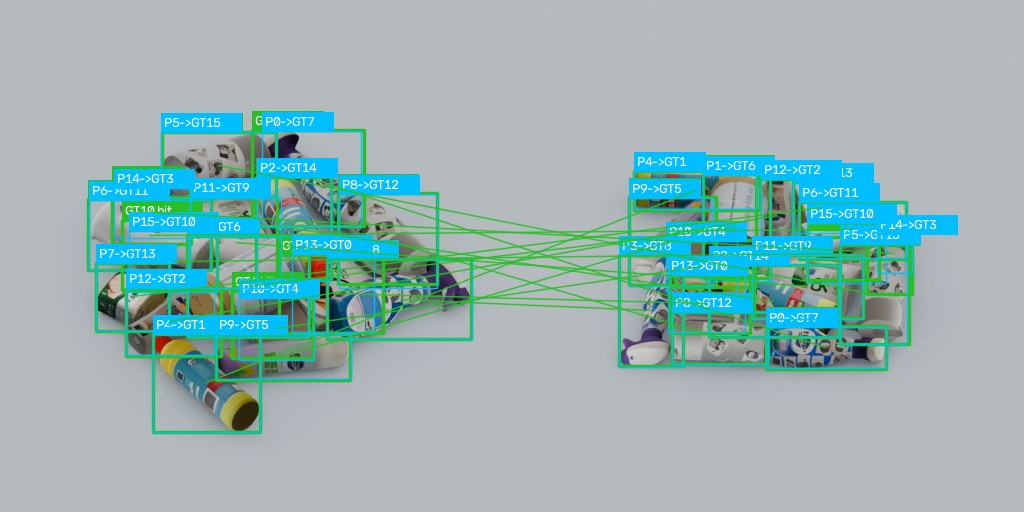
\includegraphics[width=\linewidth]{fig/scene_001001.jpg}\\[-1mm]
{\small (a) Clean example}
\end{minipage}\hfill
\begin{minipage}[t]{0.48\textwidth}\centering
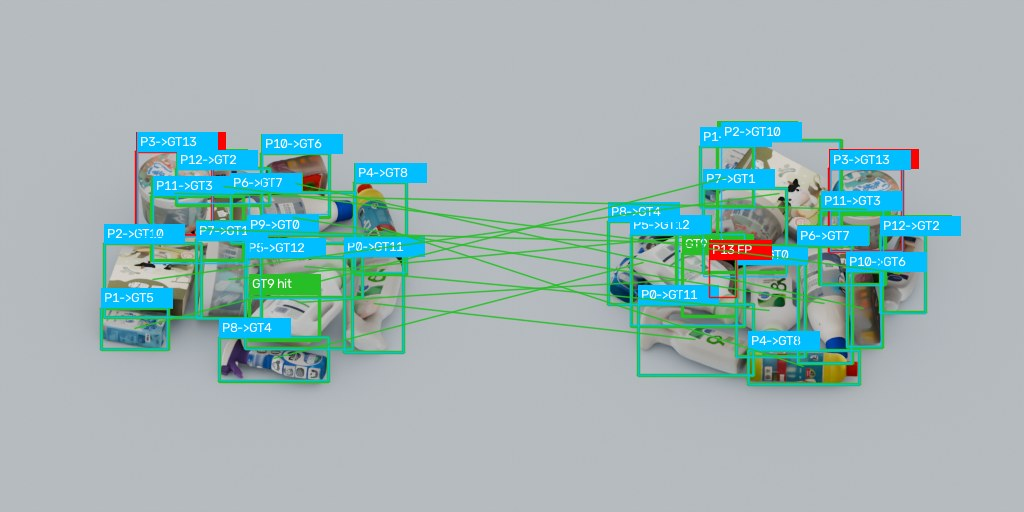
\includegraphics[width=\linewidth]{fig/scene_001000.jpg}\\[-1mm]
{\small (b) Misses and extra box}
\end{minipage}\hfill\\[2mm]
\begin{minipage}[t]{0.48\textwidth}\centering
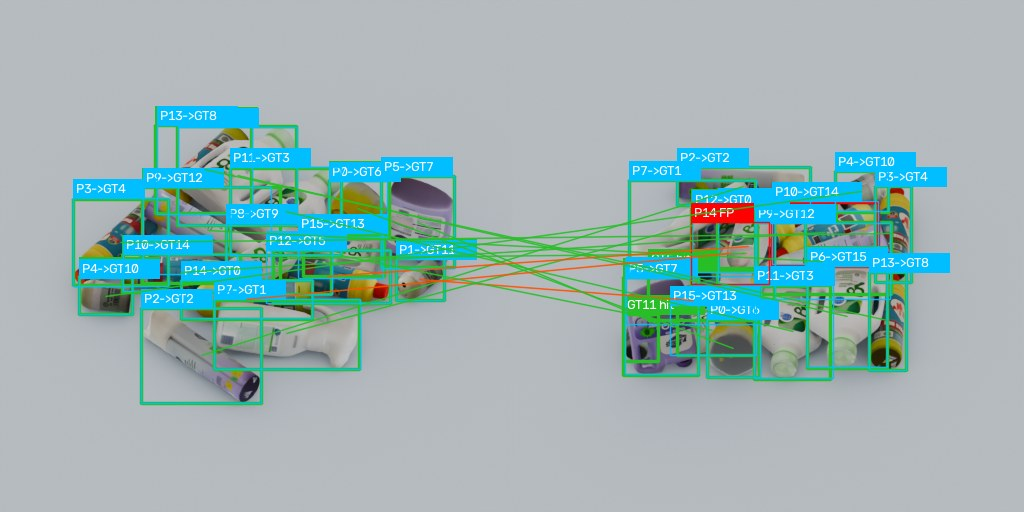
\includegraphics[width=\linewidth]{fig/scene_001002.jpg}\\[-1mm]
{\small (c) Wrong cross-view links}
\end{minipage}
\caption{Validation diagnostics from the selected scene matcher. Green outlines and links indicate correct matches; red and orange marks indicate detections or links that fail the evaluator's IoU-based matching. Each panel shows the two views of one scene.}
\label{fig:failures}
\end{figure*}

The 960-pixel detector with a learned scene-level matcher is the selected method because it gives the strongest measured balance of association and counting metrics. The experiment also shows that maximizing a single metric can be misleading: recovery marginally raises association F1, while the no-recovery model has lower count error and higher given-detection F1. Test predictions follow the required JSON structure and cover all 200 test scene pairs. Since test labels are withheld, no test accuracy is claimed. Future gains should focus on missed amodal boxes and ambiguous crowded-scene links without increasing duplicate records.
